% Chapter 1

\chapter{Time-dependent Repair Strategy} % Write in your own chapter title
\label{Chapter5}
\lhead{Chapter 5. \emph{Time-dependent Repair Strategy}} % Write in your own chapter title to set the page header
%%%

%\textbf{Keywords:} Weibull hazard function, optimal renewal interval, pipeline management.
\section{General introduction}
\label{51}
Water pipelines system in a mega city is considered as one of the most important infrastructure system of the city. Major engineering function of the system is for transportation of clean and purified water from treatment and distribution plants to various users including organizations, factories and households. Due to the limitation of land-use and social requirements, in most of the case, pipelines are placed as underground, beneath the pavements, railways and other infrastructures \cite{ahammed97}. In view of the pipeline as underground system, one of the main challenging tasks for engineer is to understand the deterioration behaviors such as: leakage occurrence, corrosion progress, wall of pipe over the time, external impact pressure, etc. This query is indeed necessary in order to efficiently operate the system so as to provide the best quality and sufficient volume of water for the city dwellers.

The main physical deteriorate problem of pipeline is corrosion resulting from many influential factors such as: internal fluid pressure, material elastic modulus, longitudinal stress, coating type, soil impact, external load and many others. Evidently, corrosion over the operation time undoubtedly and slowly leads to leakage and break of pipe. In fact, leakage occurrence and break of pipeline system in a mega city due to natural corrosive process and external factors have been well-documented as a widespread problem. As a sequent, water supply companies are asked to bear huge losses due to pressure head losses, high repair and penalty cost in case of damage occurrences. Additionally, in view of social losses, a great amount of money needs to be allocated for other potential adverse consequences such as flooding, fast deterioration of roads, road congestion, closing of business and shopping centers and other indirect expenses \cite{deb03}.

As the matter of course, data on actual performance of pipelines over the years is often absence because of its complexity and high cost in inspection. For example, the visual inspection requires excavation of existing upper structures, which therefore prevents other services from normal operation. Moreover, in the case of regular maintenance or immediate repair, the involved costs are often claimed to be considerably high. Thus, in an economical view, managers prefer to select the option of renewing the pipeline to repair alternative because the overall cost in fact receiving very small variation from material cost itself. This ideal consequently leads to the demand of determining the optimal renewal time based on the principle of minimizing the overall life cycle cost (LCC).

The determination for renewal duration is in close link not only to the overall cost but also to the durability of pipeline. Naturally, high durability pipeline is often turning to have longer optimal renewal time. In the situation of having various types of pipelines, selecting the best one that satisfies both high durability and minimum LCC requires an appropriate benchmarking study. In consideration of benchmarking, suffice to say that only when the optimal renewal duration of each pipeline type is determined, a selection of the most appropriate technology of pipelines would be feasible.

This study aims to formulating an optimal renewal model of pipeline system. Pipeline systems are subjectively categorized into different types according to the characteristics of construction materials. Each type of pipeline is further grouped by differences in diameter. Weibull hazard function is employed to address the elapsed time of each pipeline measuring from its buried time. The physical impact factors are in form of risk factor with a certain probability or range. Each impact factor results in a particular risk level and is integrated into hazard function. Expected life cycle cost considers both direct replacement cost and indirect social cost. 

The model is used for forecasting the deterioration of pipelines and determining the optimal renewal time that offers the minimum expected life cycle cost of each pipeline. The optimal types of pipeline could be identified as the best alternative for future replacement. The presumption of model is presented in the second section. The third section discusses the deterioration process of pipeline system. The best renewal interval model is portrayed in the fourth section. Empirical application to the water distribution network of Osaka city, which was established in 1895, is examined and explained in the fifth section.
%%%%%%%%%%%%%%%%%%
%\section{General Background}
%\label{52}
%%%%%%%%%%%%%%%%%%%%%%%%%%%%%%%%%%%%%%%%%%%%%%%%555
%%%%%%%%%%%%%%%%%%%%%%%%%%%%%%%%%%%%%%%%%%%%%%%%%%%
\section{Pre-assumption of the Model}
\label{53}
%%%%%%%%%%%%%%%%%%%%%%%%%%%%%%%%%%%%%%%%%%%%%%%%%%%
Suffice to say that the demand for pipeline replacement of water distribution network would not become a heavy burden if abundant resource were allocated annually. However, the scarcity of resources bring up to the managers a question of when, how and what to do for the entire network and for individual pipeline. Thus, for managerial purposes, it ought to be important not only to estimate the optimal renewal time but also the most appropriate substitute type of pipeline for present and future replacement. 

In pipeline system, there are two distinguish level of deterioration, denoting as $E_i (i=1,2)$. Level $E_1$ reflects the healthy condition in good level. Whilst, level $E_2$ denotes the pipeline is under leakage, damage or destruction. Anytime when the condition level $E_2$ is detected, the damaged pipeline will be replaced to a new one immediately. In the concurrence of incident, especially in the mega cities, tap water will spill over the surface of the road, or shopping center that lead to the social damage such as: traffic congestion, flooding and downtime of office, business center in the downtown. By substituting the old pipeline proactively, the risk of undertaking the incident could be mitigated. This is under the control and decision of Water Supply Company. As the matter of course, the substitution of pipeline demands an increase in the replacement cost. It is therefore important to harmonize the trade-off situation by introducing the optimal renewal interval with respect to the summation of total social cost and renewal cost as a whole.
\section{Deterioration Process}
\label{54}
In hazard analysis, the deterioration of element is subjected to follow a stochastic process \cite{lancaster90}. For pipeline, as previously mentioned, two condition level $E_1, E_2$ are defined. Figure \ref{fig51} describes the deterioration process of pipeline and choice of renewal. In the case of renewal, the condition state from $E_2$ must be changed into $E_1$ as for new pipeline and the pipeline resuming its normal performance condition. The renewal is carried out at alternative time $t_k$ $(k=0,1,2,...)$. In this way, the next renewal time is denoted as $t=t_0+\tau$, where $\tau$ indicating the elapsed time. The life span of the pipeline is expressed by a random variable $\zeta$. The probability distribution and probability density function of the failure occurrence are $F(\zeta)$ and $f(\zeta)$ respectively. The domain of the random variable $\zeta$ is $[0,\infty]$. The living probability (hereafter named as survival probability) expressed by survival function $\tilde{F}(\tau)$ can be defined according to the value of failure probability $F(\tau)$ in the following equation:
\begin{figure}[t]
\begin{center}
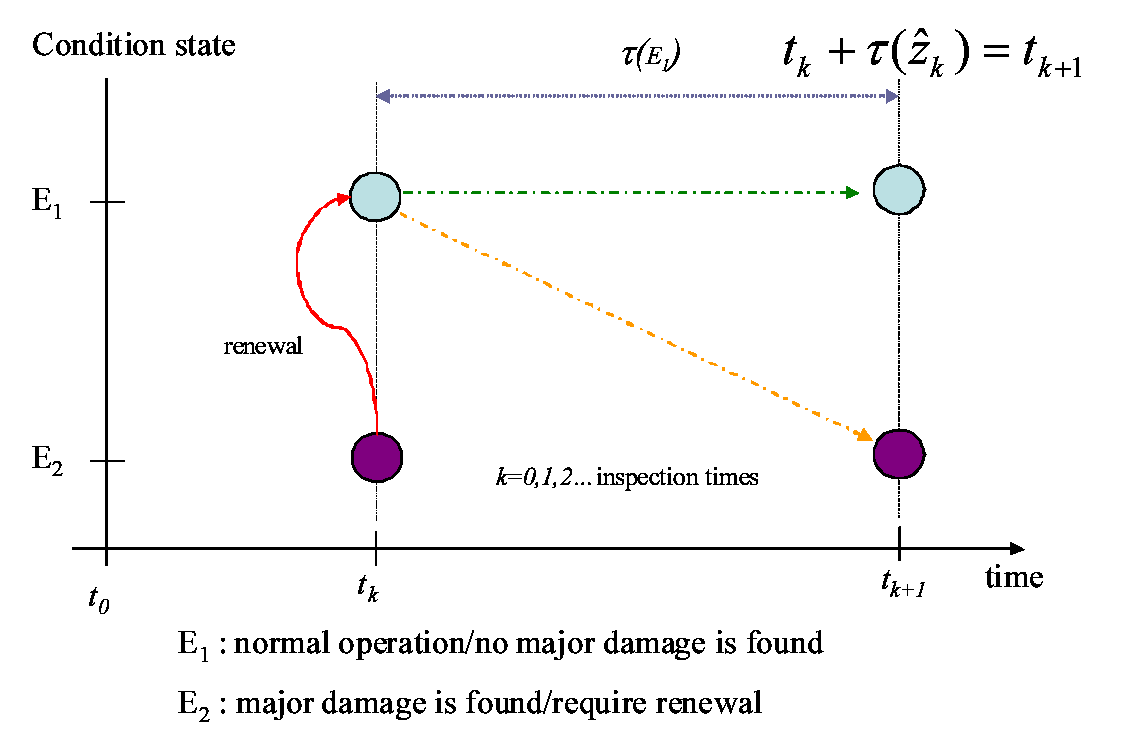
\includegraphics[scale=0.5]{fig51.eps}
\end{center}
\caption{Deterioration and Renewal Choice.}
\label{fig51} 
\end{figure}
\begin{eqnarray}
&& \tilde{F}(\tau) = 1 - F(\tau). \label{funcbF5}
\end{eqnarray}
The probability, at which the pipeline performs in good shape until time $\tau$ and break down for the first time during an interval of $\tau+\Delta\tau$ can be regarded as hazard rate and expressed in the following equation:
\begin{eqnarray}
&& \lambda_i(\tau) \Delta \tau = \frac{f(\tau)\Delta \tau}{\tilde{F}(\tau)}, \label{riskbF5}
\end{eqnarray}
where $\lambda(\tau)$ is the hazard function of the pipeline. In reality, the breakdown probability depends largely on the elapsed time of pipeline since its construction time. Thus, the hazard function should take into account the working duration of the pipelines. In another word, the memory of the system should be inherited. Weibull hazard function is satisfied in addressing the deterioration process:
\begin{eqnarray}
&& \lambda(\tau)= \alpha m \tau^{m-1}, \label{weibul}
\end{eqnarray}
where $\alpha$ is the parameter expressing the arrival density of the pipeline, and $m$ is the acceleration or shape parameter. The probability density function $f(\tau)$ and survival function $\tilde{F}(\tau)$ in the form of Weibull hazard function can be further expressed in equation (\ref{pdf}) and (\ref{survival}):
\begin{eqnarray}
&& f(\tau)=\alpha m\tau^{m-1}\exp(-\alpha \tau^m), \label{pdf} \\
&& \tilde{F}(\tau)=\exp(-\alpha \tau^m). \label{survival}
\end{eqnarray}
\section{Risk Factors and Estimation Approach for Weibull Parameters}
\label{55}
\subsection{Risk Factor and Covariates}
\label{551}
\subsubsection{Risk Factor}
\label{5511}
The corrosion process of pipeline is affected by many internal and external factors. As earlier mentioned, the influential factors include material yield stress, length, radius, pipe wall thickness, traffic load, unit soil weight, thermal expansion coefficient, internal fluid pressure and many others. These factors should be considered as either deterministic or random variables with specific mean and variance depending on the availability of gathered data and information. Evidently, these factors are proportionally contribute to the deterioration level with difference variation \cite{ahammed95,ahammed97}. It is therefore, it is understandable to propose an integrated risk factor $\kappa$ in form of probability value. This risk factor receives different value in the case of different mega city, different type of water distribution system, materials and so on and so fourth. Estimation of risk factor can be retrieved from several physical models. Further expression of hazard function whereby considering the risk factor $\kappa$ is as follow:
\begin{eqnarray}
&& \lambda(\tau)= \kappa \alpha m \tau^{m-1}. \label{weibul1}
\end{eqnarray}
The probability density function $f(\tau)$ in (\ref{pdf}) and survival function in (\ref{survival}) $\tilde{F}(\tau)$ are further expressed as
\begin{eqnarray}
&& f(\tau)=\kappa \alpha m\tau^{m-1}\exp(-\kappa \alpha \tau^m), \label{pdf1} \\
&& \tilde{F}(\tau)=\exp(-\kappa \alpha \tau^m). \label{survival1}
\end{eqnarray}
A further notice in the case of using the risk factor is that $\kappa$ should be used for respective record available in the data set.
\subsubsection{Covariates}
\label{5512}
Beside the risk factor, another popular approach in addressing the impacts and correlations of characteristic variables (or covariates) is to consider location parameter $\alpha$ in additive form of covariates:
\begin{eqnarray}
\alpha  = \sum\limits_{i = 1}^M {\beta _i x_i \rm{  \hspace{2mm}   (i = 1,}}...{\rm{,M)}}, \label{covariate}
\end{eqnarray}
where $m$ is total number of covariates and the value of first covariate equals to 1 as a constant value. Depending the availability of database, numbers of covariates are selected in to numerical calculation.
\subsection{Estimation Approach for Weibull Parameter}
\label{552}
It is assumed that the total number of recorded data is $S$, which is relatively equivalent to entire length of the pipelines system. In which, each record refers particularly for $s$ $(s=1,...,S)$ unit of length (possibly in meter or kilometer). This type of separation is often found for the convenience of management of each city. Equations (\ref{pdf}) and (\ref{survival}) are thus in the following formula:
\begin{eqnarray}
&& f(t_s)=\alpha mt_s^{m-1}\exp(-\alpha t_s^m), \\
&& \tilde{F}(t_s)=\exp(-\alpha t_s^m).
\end{eqnarray}
%%%%%%%%%%%%%%%%%%%
Deterioration of section $s$ is considered as mutually independent from other part of the pipelines system. For this reason, the simultaneous probability density of the deterioration is expressed in the following likelihood function: 
%%%%%%%%%%%%%%%%%%%%%
\begin{eqnarray}
\begin{array}{l}
 {\cal L} (\alpha , m: t_s) = \prod\limits_s^S {\left\{ {\bar F(t_s^m )} \right\}^{(1 - \delta _s )} \left\{ {f(t_s^m )} \right\}^{\delta _s } }    \\
= \prod\limits_s^S {\left\{ {\exp ( - \alpha t_s^m )} \right\}^{(1 - \delta _s )} \left\{ {\alpha mt_s^{m - 1} \exp ( -  \alpha t_s^m )} \right\}^{\delta _s } } , \label{eq11}
 \end{array}
\end{eqnarray}
where $\delta_s$ is dummy variable receiving its value of $1$ when leakage was encountered and $0$ otherwise. For ease of mathematical manipulation, logarithm for both sides of equation (\ref{eq11}) is referred. Thus, following equation is additional named as log-likelihood function:
\begin{eqnarray}
&&\ln {\cal L} (\alpha, m: t_s )=  
\sum\limits_s^S {\left[ \begin{array}{l}
 (1 - \delta _s )( - \alpha t_s^m ) \\ 
  + \delta _s \left\{ {\ln \alpha  + \ln m + (m - 1)\ln t_s  - \alpha t_s^m } \right\} \\ 
 \end{array} \right]} .\label{weilike}
\end{eqnarray}
In order to obtain the two parameter $\alpha$ and $m$, the maximum likelihood estimation method is used. The estimator of parameter value $\theta$ which maximizes the logarithmic likelihood function (\ref{weilike}) is given as $\hat\theta =(\hat \theta _1 ,\hat\theta _2)$ ($\theta _1 =\alpha, \theta _2 =m $) and must simultaneously satisfies following condition:
\begin{eqnarray}
\frac{{\partial \ln {\cal L} (\Xi ,\hat \theta )}}{{\partial \theta _i }} = 0,{\rm{      }}(i = 1,2) .
\end{eqnarray}
Furthermore, the estimated value $\sum {\hat \theta }$ of the asymptotic covariance matrix of the parameter can be expressed as follow:
\begin{eqnarray}
\sum\limits_{}^ \wedge  {(\hat \theta ) = \left[ {\frac{{\partial \ln {\cal L} (\Xi ,\theta )}}{{\partial \theta \partial \theta^{'} }}} \right]} ^{ - 1} . \label{fisher}
\end{eqnarray}
%%%%%%%%%
The optimal value of $\hat\theta =(\hat \theta _1 ,\hat\theta _2)$ are then estimated by applying numerical iterative procedure such as Newton method for simultaneous equation (\ref{fisher}) of 2 dimensions. This study employs Newton-Rhapson method. The statistical $t$-test is calculated by use of covariance matrix value $\sum {\hat \theta }$.
%%%%%%%%%%%%%%%%%%%%%%%%%%%%%%%%%%%%%%%%%
\section{Formulation of the Optimal Renewal Interval Model}
\label{56}
The occurrence of the incident results in an amount of social cost, which is assumed to be a constant number $C$. The expected social cost $EC(z)$ is estimated by use of the predetermined interval of renewal $z$. Thus, its value is followed the probabilistic manner via probability density function $f(\tau)$ defined in equation (\ref{pdf}). Over the continuous time, counting from the buried time or the previous renewal time, the expected social cost would be in the integral form as expressed in the following equation:
\begin{eqnarray}
&& EC(z)=\int_0^{z} C f(t)\exp(-\rho t)dt. \label{socialcost}
\end{eqnarray}
The co-efficient $\rho$ is discounted rate of money over the interval $z$. On the other hand, another constant amount of money denoted as $I$ is spent for renewal activities, which is subjected to either occurrence of incident at time $\tau$ or the age of pipeline reaching to time $z$. It is therefore important to note that the renewal cost, when the age of pipeline becomes $z$, must take the survival probability $\tilde{F}(\tau)$ into its calculation. Consequently, the present discounted cost of the next pre-determined renewal time $EL(z)$ can be expressed in the following form:
\begin{eqnarray}
EL(z)=\int_0^{z} I f(t)\exp(-\rho t)dt +  \tilde{F}(z)I \exp(-\rho z). \label{totalcost}
\end{eqnarray}
The expected life cycle cost after the next renewal time is evaluated as net present value of social costs, renewal costs. As the social and renewal cost are in fixed values, the expected LCC alters to be equal for every renewal times. In another word, expected LCC at next renewal time is equal to the expected LCC estimated at the present renewal. The expected LCC, denoted as $J(0:z)$, can be regulated through the regression estimation shown in equation (\ref{han}):
\begin{eqnarray}
&& J(0:z)= \int_0^{z} f(t)\{c+I+J(0:z)\} \exp(-\rho t)dt  \nonumber \\
&& \hspace{10mm} + \tilde{F}(z)\{I+J(0:z)\} \exp(-\rho z).  \label{han}
\end{eqnarray}
The following two functions $\Gamma(z)$ and $\Lambda(z)$ are defined:
\begin{eqnarray}
&& \Gamma(z)=\int_0^{z} f(t)\exp(-\rho t)dt 
 = \int_0^z  \alpha m\tau^{m-1}\exp(- \alpha \tau^m-\rho t)dt, \label{gamma5}\\
&& \Lambda(z)= \tilde{F}(z) \exp(-\rho z)
  =\exp(- \alpha z^m-\rho z) . \label{alpha}
\end{eqnarray}
Substituting equations (\ref{gamma5}) and (\ref{alpha}) into equation (\ref{han}), the following explicit form for the expected LCC is obtained:
\begin{eqnarray}
&& J(0:z)= \frac{(c+I)\Gamma(z)+I \Lambda(z)}{1-\Gamma(z)-\Lambda(z)} .\label{lifecycle}
\end{eqnarray}
The optimal value function $\Phi(0)$ can be expressed as the minimum expected LCC evaluated at the initial time:
\begin{eqnarray}
&& \Phi(0)=\min_{z}\{ J(0:z) \}.\label{imp}
\end{eqnarray}
The estimation for the optimal interval $z^*$ from equation (\ref{lifecycle}) can be handled by solving the optimization condition of the first derivative as expressed in the following equation:
\begin{eqnarray}
&& \frac{dJ(0:z)}{dz}=\frac{ \psi(z)}{\{1-\gamma(z)-\Lambda(z)\}^2 }=0, \\
\text{where}\nonumber \\
&& \psi(z)=(C+I)\Gamma^\prime(z)+I\Lambda^\prime(z)+C\{\Lambda(z)^\prime\Gamma(z)
 -\Gamma^\prime(z)\Lambda(z)\},
\end{eqnarray}
$\Gamma(z)^\prime=d\Gamma(z)/dz$ and $\Lambda(z) ^\prime=d\Lambda(z)/dz$. Obtaining the value of optimal interval $z^*$ requires to solve the equation $\psi(z)=0$. Another numerical approach to solve equation (\ref{lifecycle}) is further explained in appendix A.
%%%%%%%%%%%%%%%%%%%%%%%%%%%%%%%%%%%%%%%%%%%%%%%%%%%%%%%%
\section{Optimal Renewal Interval and Technology Innovation}
\label{57}
The water distribution network composes of many different types of pipes. Thanks to the technology innovation in pipe's materials, many new and better quality types of pipe have been introduced. As a matter of course, along the time, pipelines made from outdated materials are no longer in production. The aging pipelines are deeming to be substituted by better quality pipes. It is assumed that the network composes of type $i$ $(i=1,...,N)$, which is available in the stock ($N$ is total number of type $i$). On the other hand, there exists pipes of old fashion type $j$ $(j=1,...,M)$ ($M$ is the total number of old type). The selection of pipe according to its type for renewal activities can be described in two subsequent steps as follows:
%%%%%%%%%%%%%%%%%%%%%%%%%%%%%%%%%%%%%%%%%%%%%%%
\subsection{Step 1-Selection of Best Type of Pipe}
\label{571}
The optimization approach expressed in equation (\ref{lifecycle}) and (\ref{imp}) warrants the estimation for the best interval renewal time for each type $i$ $(i=1,...,N)$ of pipelines. From equation (\ref{han}), the following equation is regarded as the expected LCC for type $i$:
\begin{eqnarray}
&& J_i(0:z_i)= \int_0^{z_i} f_i(t)\{c+I_i+J_i(0:z_i)\} \exp(-\rho t)dt  \nonumber \\
&& \hspace{10mm} + \tilde{F}_i(z_i)\{I+J_i(0:z_i)\} \exp(-\rho z_i).  \label{han1}
\end{eqnarray}
The best type $i^*$ is the one meeting the minimum expected LCC condition among $N$ types:
\begin{eqnarray}
&& i^\ast=\mbox{arg} \min_{i}\{J_i(0:z_i):i=1,\cdots,N\}. \label{16}
\end{eqnarray}
The sign $\mbox{arg}\min_{i}$ denotes the minimization searching for the function in the parenthesis with respect to $i$. The best type $i^*$ evaluated from condition of equation (\ref{16}) would become optimal type for replacement of old types of pipelines in the entire water distribution network.
%%%%%%%%%%%%%%%%%%%%%%%%%%%%%%%%%%%%%%%%%%%%%%%
\subsection{Step 2-Replacement for Old Type Pipeline}
\label{572}
In regard to replacement rules, the expected life cycle $\tilde{J}_j^{i^\ast} (z_j:\tau_j)$ cost calculated for the old type $j$ of pipe by using the optimal type $i^*$ acquired from Step 1 and after interval time $z_j$ become the net present value expressed in the following equation:
\begin{eqnarray}
&& \tilde{J}_j^{i^\ast}(z_j:\tau_j)
 =\int_0^{z_j} f_j(t_j|\tau_j)\{c+I_{i^\ast}+J_{i^\ast}(0:z_{i^\ast})\} \exp(-\rho t_j)dt_j  \nonumber \\
&& + \tilde{F}_j(z_j|\tau_j)\{I+J_{i^\ast}(0:z_{i^\ast})\} \exp(-\rho z_{i^\ast}) . \label{han2}
\end{eqnarray}
The problem of seeking for the optimal renewal time $z_j^\ast(\tau_j)$ for old type $j$ with elapsed time $\tau$ is by solving the optimization condition in the following expression:
\begin{eqnarray}
&& z_j^\ast=\arg \min_{z_j} \{\tilde{J}_j^{i^\ast}(z_j:\tau_j)\} .\label{sa}
\end{eqnarray}
%%%%%%%%%%%%%%%%%%%%%%%%%%%%%%%%%%%%%%%%%%%%%%
%%%%%%%%%%%%%%%%%%%%%%%%%%%%%%%%%%%%%%%%%%%%%%
The so called \textit{"Switching ratio $\Theta$" }, inferring the rate of renewal by using the new type of pipelines over the old types, is expected to become an important indicator for replacement planning. Definition of the rate is the ratio of $z^*_j$ over $z^*_i$:
%%%
\begin{eqnarray}
&& \Theta = \dfrac{z^*_j}{z^*_i} .\label{swratio}
\end{eqnarray}
%%%%
\section{Average Cost Estimation.}
The application of average life cycle cost analysis has been widely recommended for economic evaluation of public infrastructure, Especially, for infrastructure with its long service life. This is due to the fact that, over the years, discount rate $\rho$ often exerts a high fluctuation in its value. In order to minimize the negative impact on analysis from such high fluctuation of discount rate, \cite{kobaevarg} has proved the benefit of using average cost analysis.

The case when life cycle cost is applicable is in line with the case when the denominator of the expression \ref{lifecycle} becomes $0$ in the limit of which discount rate $\rho=0$. However, when the value of denominator equals to $0$, the equation can not be solvable. In consideration average cost over the service life, we apply estimation for average cost of pipeline type $i~(i=1,\cdots,N)$ by following equation:
\begin{eqnarray}
&& AC_i(z)=\frac{\int_0^{z} (c+I_i) f_i(t) dt  +  \tilde{F}_i(z)I_i}{z} .\label{avelcc}
\end{eqnarray}
The optimal renewal time $z_i^\ast$ for pipeline type $i$ can be estimated by solving the minimum condition of equation \ref{avelcc}:
\begin{eqnarray}
&& \min_{z}\{ AC_i(z) \}.\label{iimp}
\end{eqnarray}
Among $N$ number of type $i$, again, it is possible to select the best type $i^\ast$ in view of least life cycle cost:
\begin{eqnarray}
&& i^\ast=\mbox{arg} \min_{i}\{ AC_i(z_i^\ast):i=1,\cdots,N\}.
\end{eqnarray}
Eventually, it is possible to define the average cost if the best pipeline type $i^\ast$ is used to replace the old type of pipeline $j$. And thus, it is necessary to define the renewal period $z_j$ in case of renewal with best possible pipeline technology:
\begin{eqnarray}
&& \hspace{-5mm} \overline{AC}_j^{i^\ast}(z_j)
  =\frac{\int_0^{z_j} f_j(t_j|\tau_j)(c+I_{i^\ast}) dt_j  + \tilde{F}_j(z_j|\tau_j)I_{i^\ast} }{z_j} .\label{han11}
\end{eqnarray}
$\tilde{F}_j(t_j|\tau_j)$ is the probability, to which, leakage or breakdown do not occur during time $t_j$ and continue the same condition state until time $\tau_j$. If the best pipeline type $i^\ast$ now is used, the average cost $AC_{i^\ast}(z_i^\ast)$ is generated. In addition, the accumulative additional cost generated by continuously using the old pipeline for the $z_j$ period can be determined:
\begin{eqnarray}
&& \overline{CAC}_j^{i^\ast}(z_j)= \{\overline{AC}_j^{i^\ast}(z_j)-AC_{i^\ast}(z_i^\ast)\}z_j.
\end{eqnarray}
In the end, the best renewal time $z_j^\ast(\tau_j)$ for pipeline type $j$ can be easily estimated by choosing the renewal time satisfying the minimum condition: 
\begin{eqnarray}
&& z_j^\ast=\arg \min_{z_j} \{\overline{CAC}_j^{i^\ast}(z_j)\}. \label{ssa}
\end{eqnarray}
\section{Empirical Study}
\label{58}
\subsection{Overview of Empirical Study}
\label{581}
%%%%%%%%%%%%%%%%%%%%%%%%%%%%%%%%%%%%%%%%%%%%%%
The water distribution network of Osaka city was mainly constructed during the periods of 1950s and 1960s. The network has undergone nice times of expansion to meet the need of the city \cite{osaka}. The total length of conduct, transmission and distribution pipe is approximately 5,000 km. Since 1965, the City has systematically upgraded the distribution system by installing new pipes, renewing aged ones, lining all pipes, etc. As a result, a network of distribution pipes in the city has been satisfactorily established, eliminating insufficient supply and low water pressure supply areas. To date, the subsequent maintenance and renewal activities have been so far implemented for over $4,000$ km, requiring about more than $390$ billion Japanese Yen.

Technically, the entire water distribution system composes of four distinguish types, which belongs to class A, C, F and FL. The three types C, F and FL are the old cast iron types, which were buried in the early period. At the present, those pipes are no longer in the manufacturing. As the matter of course, the social cost $C$, direct cost $I$ and discounted rate $\rho$ plays a center role in establishing the optimal renewal years as well as the expected LCC, sensitivity analysis with focus on the ranges are drawn for respective types of pipelines. However, for ease of estimation, benchmark case was selected with social cost $C=5$ million Yen, $I =1$ million Yen and $\rho=0.04$.%%%%%%%%%%%%%%%%%%%%%%%%%%%%%%%%%%%%%%%%%%%%%%
\subsection{Estimation Results}
\label{582}
\subsubsection{Weibull's parameters and survival probability}
\label{5821}
%%%%%%%%%%%%%%%%%%%%%%%%%%%%%%%%%%%%%%%%%%%%%%
The parameters $\alpha$ and $m$ of embedded hazard function are estimated by maximum likelihood method with historical sectional records for each type of pipeline. Values of $\alpha$ and $m$ are then verified with significant degree of $t$ test values. Table \ref{table51} presents the results of estimation for two comparative cases. The first case refers as case, to which explanatory variables were excluded from estimation. Second case were when the effective length as characteristic variable was considered in estimation. Regarding the second case, as presented in the table, unknown parameter $\beta_1$ is referred to a constant term with its value of $1$ for characteristic variable $x_1$. Unknown parameter $\beta_2$ is referred to the effective length of pipeline system. 

In this study, other characteristic variables, which reflect the influence of outer and inner rutness, soil unit weight, top traffic volume, etc, were neglected due to its small impact or data unavaibility. The value in blankets in Table \ref{table51} refers to value of statistical $t-test$. It is realized from $t-test$ value that effective length of pipeline somehow effect the deterioration process. This conclusion is further understandable from comparison of AIC \footnote{AIC-Akaike Information Criteria was developed by Hirotsugu Akaike, a Japanese statistician, in 1971. The AIC is not test on the model in the sense of hypothesis testing, rather it is a tool for model selection.} (Akaike Information Criteria)  \cite{akaike} values. AIC values of case with considering effective length of pipeline are lower than the case without that covariate in estimation (AIC values are shown in the last line of each row in Table \ref{table51}).
%
\begin{table}[t]
\caption{Estimation Results for the Parameters of Weibull Functions-Types}
\label{table51}
{\small
\begin{center}
\begin{tabular}{l|ll|lll}
\hline
\multicolumn{1}{c|}{Pipeline} & \multicolumn{2}{c|}{Without covariate} & \multicolumn{3}{c}{With covariate} \\ 
\multicolumn{1}{c|}{types} & \multicolumn{1}{c}{$\alpha$} & \multicolumn{1}{c|}{m} & \multicolumn{1}{c}{$\beta_1$} & \multicolumn{1}{c}{$\beta_2$} & \multicolumn{1}{c}{m} \\ 
\hline
\multicolumn{1}{c|}{C} & \multicolumn{1}{c}{1.11E-05} & \multicolumn{1}{c|}{2.496} & \multicolumn{1}{c}{2.51E-06} & \multicolumn{1}{c}{1.49E-04} & \multicolumn{1}{c}{2.484} \\ 
\multicolumn{1}{c|}{} & \multicolumn{1}{c}{(28.528)} & \multicolumn{1}{c|}{(30.275)} & \multicolumn{1}{c}{(6.402)} & \multicolumn{1}{c}{(19.666)} & \multicolumn{1}{c}{(34.909)} \\ 
\multicolumn{1}{c|}{} & \multicolumn{2}{c|}{5053.724 } & \multicolumn{3}{c}{4,031.920 } \\ 
\hline
\multicolumn{1}{c|}{F} & \multicolumn{1}{c}{2.55E-05} & \multicolumn{1}{c|}{2.293} & \multicolumn{1}{c}{4.92E-06} & \multicolumn{1}{c}{3.25E-04} & \multicolumn{1}{c}{2.288} \\ 
\multicolumn{1}{c|}{} & \multicolumn{1}{c}{(46.256)} & \multicolumn{1}{c|}{(48.825)} & \multicolumn{1}{c}{(9.337)} & \multicolumn{1}{c}{(32.944)} & \multicolumn{1}{c}{(56.613)} \\ 
\multicolumn{1}{c|}{} & \multicolumn{2}{c|}{13,523.840 } & \multicolumn{3}{c}{11,154.640 } \\ 
\hline
\multicolumn{1}{c|}{FL} & \multicolumn{1}{c}{1.81E-05} & \multicolumn{1}{c|}{2.400} & \multicolumn{1}{c}{6.73E-06} & \multicolumn{1}{c}{1.22E-04} & \multicolumn{1}{c}{2.391} \\ 
\multicolumn{1}{c|}{} & \multicolumn{1}{c}{(14.537)} & \multicolumn{1}{c|}{(15.432)} & \multicolumn{1}{c}{(4.375)} & \multicolumn{1}{c}{(7.365)} & \multicolumn{1}{c}{(17.790)} \\ 
\multicolumn{1}{c|}{} & \multicolumn{2}{c|}{1,331.980 } & \multicolumn{3}{c}{1,114.080 } \\ 
\hline
\multicolumn{1}{c|}{A} & \multicolumn{1}{c}{8.87E-05} & \multicolumn{1}{c|}{1.907} & \multicolumn{1}{c}{8.27E-06} & \multicolumn{1}{c}{4.18E-04} & \multicolumn{1}{c}{2.144} \\ 
\multicolumn{1}{c|}{} & \multicolumn{1}{c}{(29.416)} & \multicolumn{1}{c|}{(31.380)} & \multicolumn{1}{c}{(10.117)} & \multicolumn{1}{c}{(26.642)} & \multicolumn{1}{c}{(35.865)} \\ 
\multicolumn{1}{c|}{} & \multicolumn{2}{c|}{6,654.540 } & \multicolumn{3}{c}{5,588.270 } \\ 
\hline
\end{tabular}
\end{center}
}
{\small Note) Value in the blanket $(-)$ are stasitical t-test. Values in the last row of each type are $AIC$ values.}
\end{table}%[t]
%

%Further to the value of $t-value$ for statistical test, Akaike Information Criteria (AIC) test is highly recommended to have more comprehensive understanding on the correlation of model's parameters \cite{akaike}. Formula for AIC is as follows.
%\begin{eqnarray}
%&& AIC = -2*ln(likelihood)+2*K \label{aic}
%\end{eqnarray}
%where $K$ is the number of parameters in the model. As can be seen from Table 2, the ratios of important weight $w_i$ of case 3 and case 4 receive significant small. This proves the fact that their correlation between these two factors can be neglected. From $t-value$ and AIC value, confidently to say, omission of effective length and rut is acceptable in model's calculation. However, other factors such as traffic volume above the pipelines, unit weight of soil, various type of pressure should be recommended as covariates only if the concerning data are available.
However, as can be proved from Figure \ref{fig52}, Figure \ref{fig53} and Figure \ref{fig54}, the difference in decrease of survival probability over the years are not significant for both cases of pipeline type C, F and FL. A considerable variation between two survival probability curve is realized only for pipeline type A from Figure \ref{fig55}. Since the largest sampling population has been accumulated for pipeline type A (about more than 15,000 data), it can be concluded that, the impact of effective pipeline length has tendency to increase with the larger size of sampling population. 

\begin{figure}[t]
\begin{center}
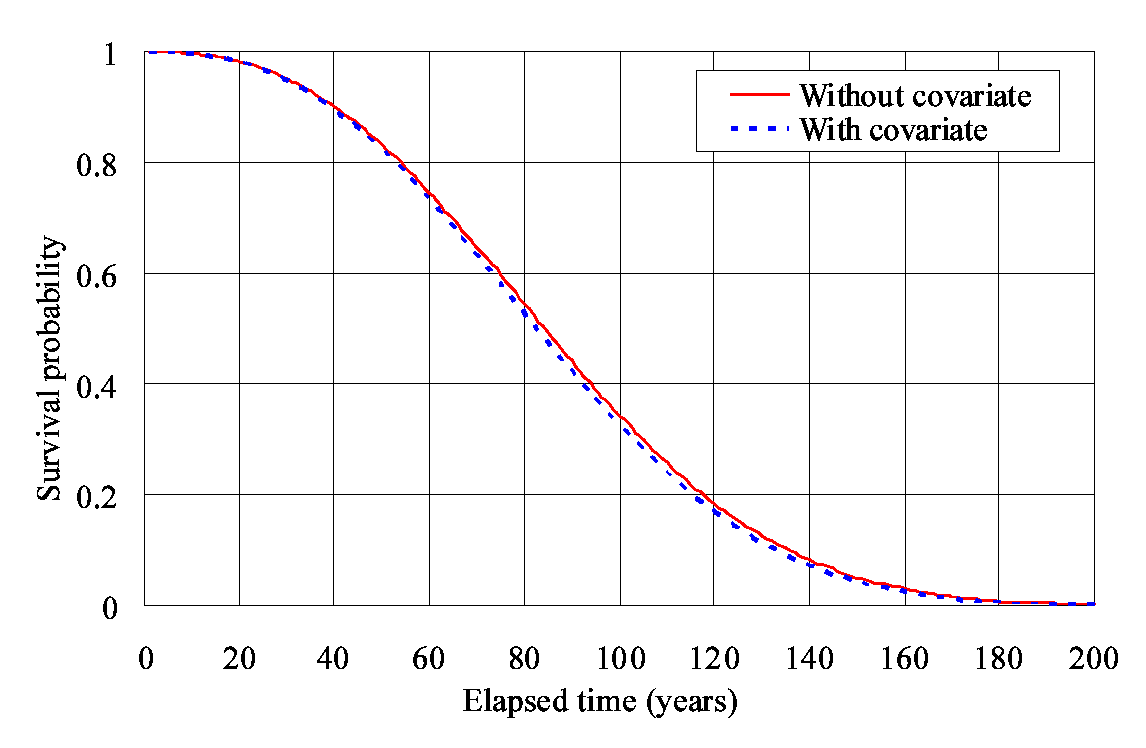
\includegraphics[scale=0.5]{fig52} 
\end{center}
\caption{Survival Probabilities of Type C With and Without Covariates.}
\label{fig52} 
\end{figure}
%
\begin{figure}[t]
\begin{center}
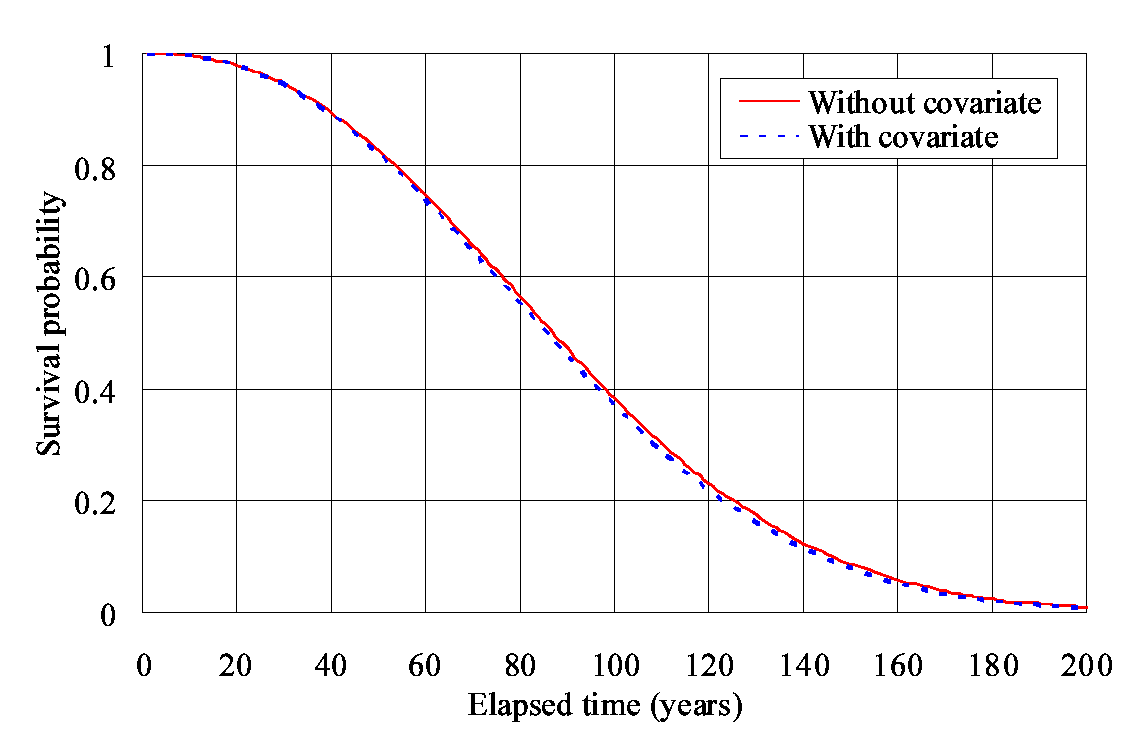
\includegraphics[scale=0.5]{fig53} 
\end{center}
\caption{Survival Probabilities of Type F With and Without Covariates.}
\label{fig53} 
\end{figure}
%
\begin{figure}[t]
\begin{center}
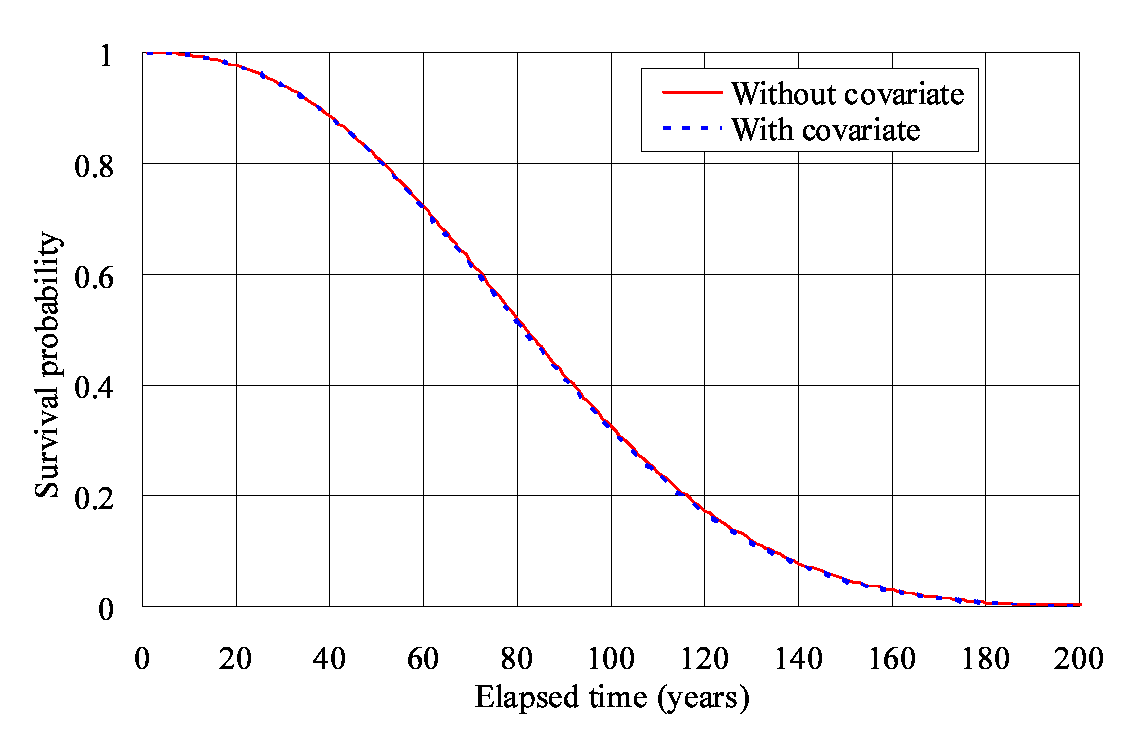
\includegraphics[scale=0.5]{fig54} 
\end{center}
\caption{Survival Probabilities of Type FL With and Without Covariates.}
\label{fig54} 
\end{figure}
%
\begin{figure}[t]
\begin{center}
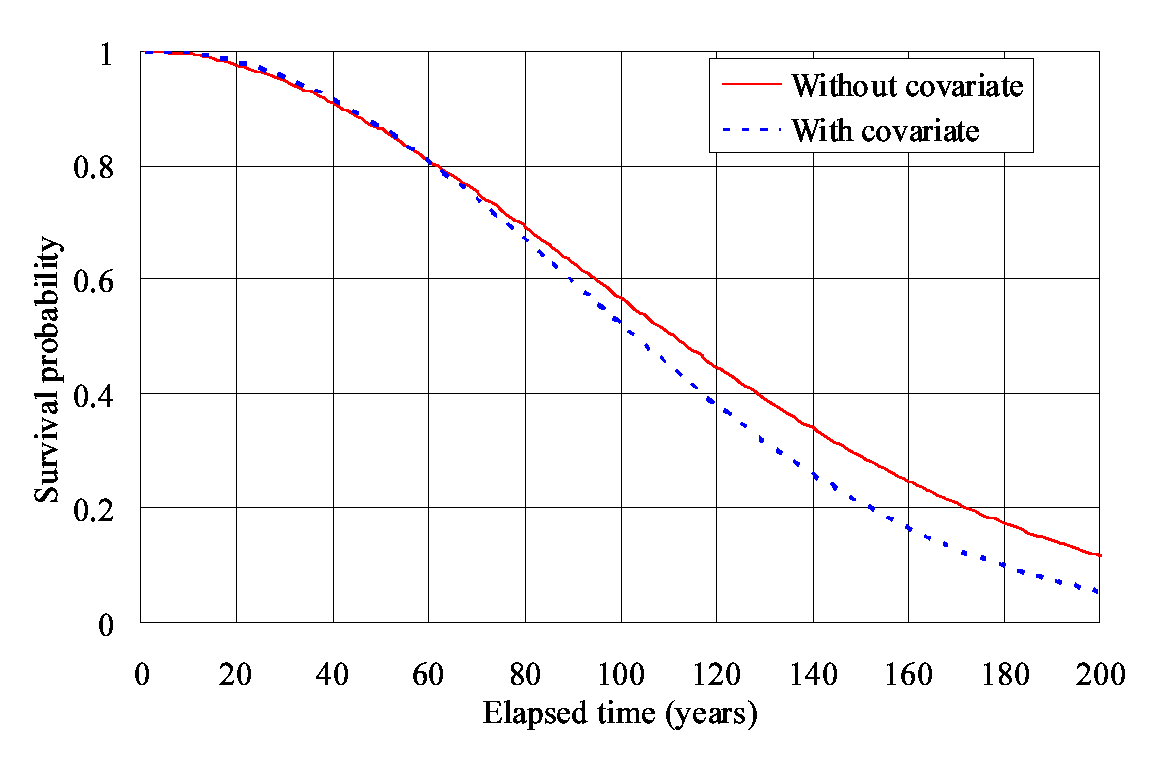
\includegraphics[scale=0.5]{fig55} 
\end{center}
\caption{Survival Probability of Type A With and Without Covariates.}
\label{fig55} 
\end{figure}
%%%%%%%%%%%
A comparative look in the survival probability curve of each pipeline type is drawn in Figure \ref{fig56}. As can be seen from the figure, pipeline type C and FL have faster decrease than pipeline type F. However, all three old pipeline types exert to has $0.5$ probability of being broken after 80 years in operation. On the other hand, pipeline type A deems to has much longer life expectancy than the others.
\begin{figure}[t]
\begin{center}
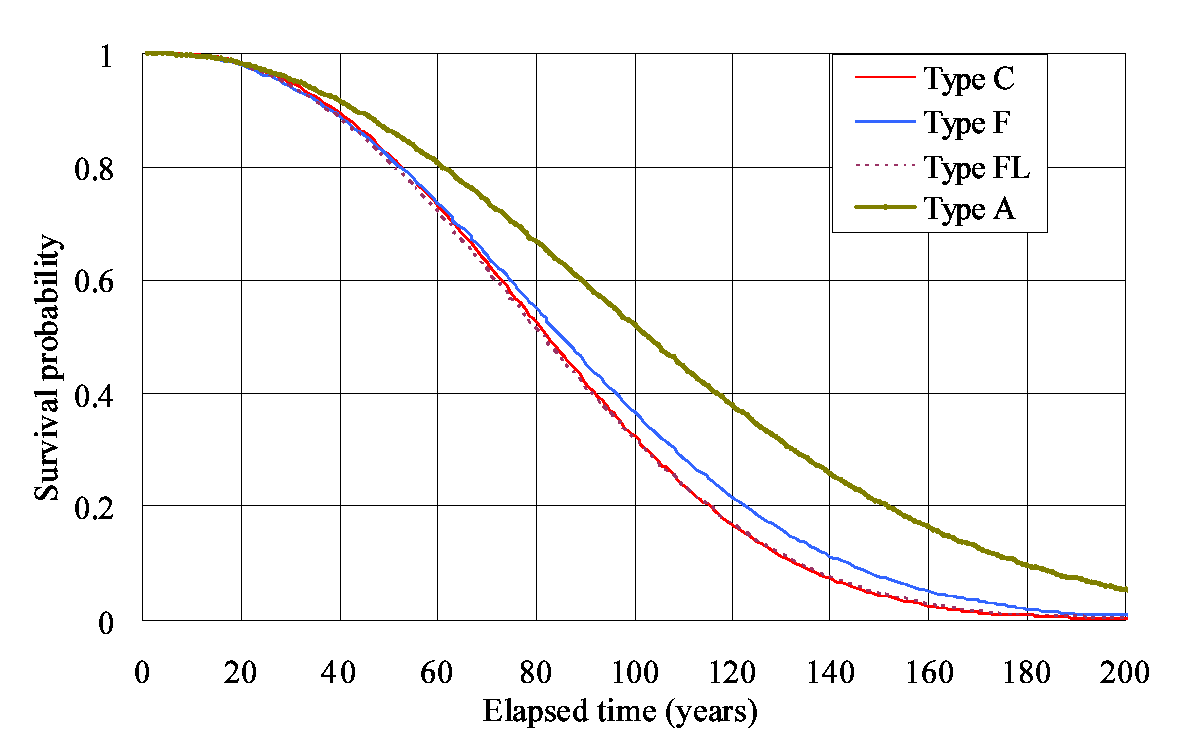
\includegraphics[scale=0.5]{fig56} 
\end{center}
\caption{Survival probabilities among Different Types of Pipelines.}
\label{fig56} 
\end{figure}
%
\subsubsection{Optimal renewal time and expected life cycle cost}
\label{5822}
Estimation for optimal renewal time and expected life cycle cost is carried out in the second phase after obtaining the values for Weibull's parameters and the associate costs. Minimization principle to seek for the optimal duration $z^*$ is empirical analyzed by using equations (\ref{han1}- \ref{sa}). Results of estimation are presented in Figure \ref{fig57} for benchmark case ($C$ = $5$ million Yen for social cost, $I=1$ million Yen for direct repair cost and $\rho=0.04$ for discount rate). It ought to recognize that the optimal renewal duration is in the range of 50 to 60 years for old types of pipelines and about 80 years of optimal renewal duration for type A.
\begin{figure}[t]
\begin{center}
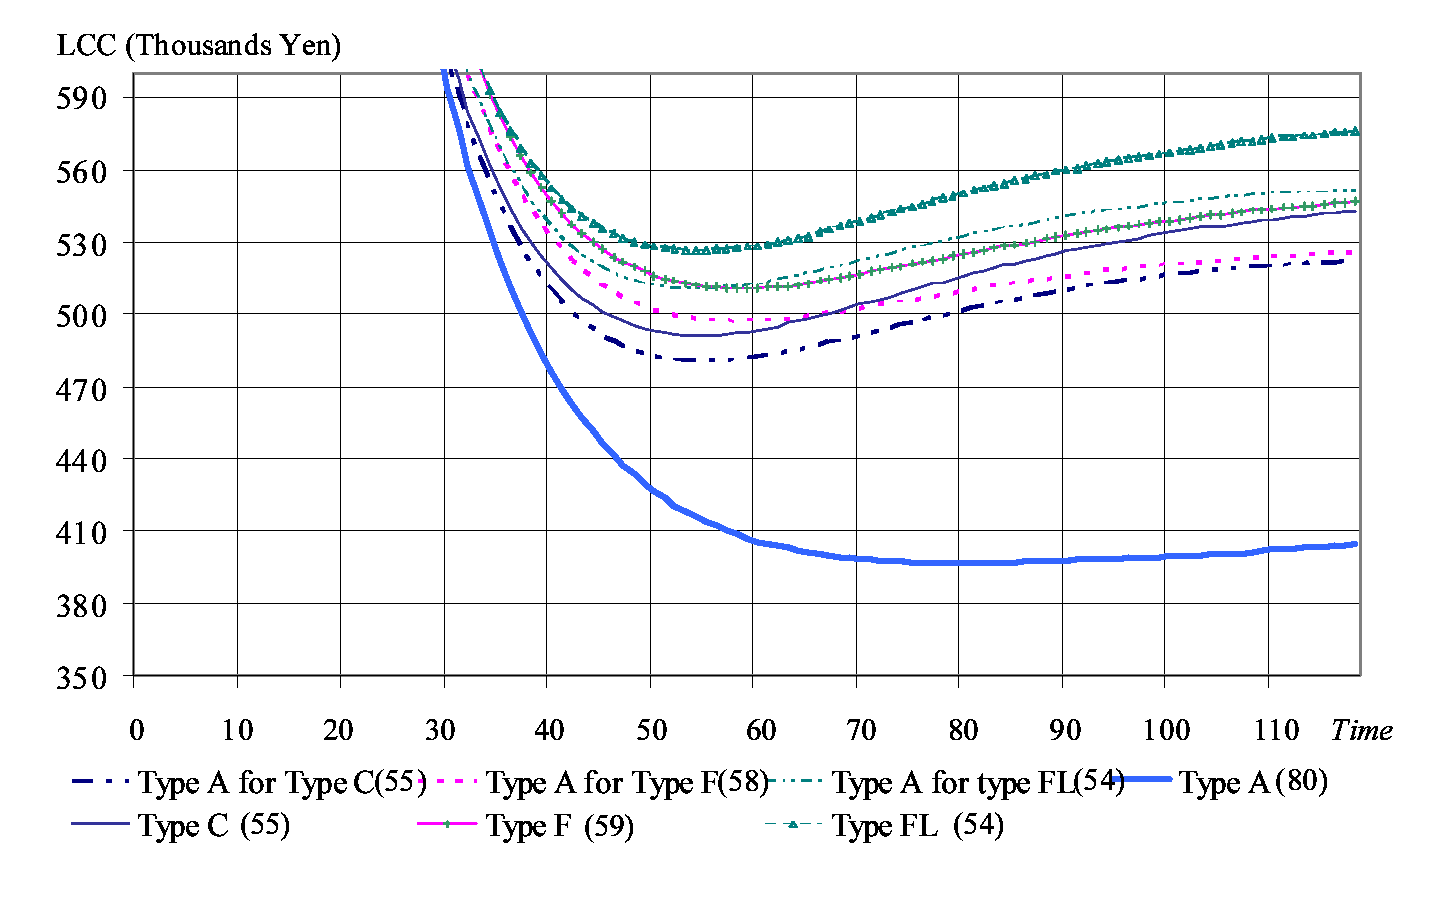
\includegraphics[scale=0.5]{fig57} 
\end{center}
\caption{Comparision of Expected Life Cycle Cost with Switching Curves.}
\label{fig57} 
\end{figure}
%%%%%%%%%%%%%%%%%%%%%%%%%%%%%%%%%%%%%%%%%%%%%%
%%%%%%%%%%%%%%%%%%%%%%%%%%%%%%%%%%%%%%%%%%%%%%
\subsubsection{Switching Rate}
\label{5823}
Figure \ref{fig57} further describes the changes of LCC for respective old types of pipelines when using type A for replacement. In this case, the optimal renewal years yield slightly shorter than if using the old types of pipeline. For example, if using type A to replace type F, the optimal renewal duration is 59 years instead of 58 years. Based on the definition in equation (\ref{han2}), the switching rate for type C, F and FL are ($\Theta_{A-C}=55/55=1.000$), ($\Theta_{A-F}=58/59=0.983$), ($\Theta_{A-FL}=54/55=0.981$) respectively.
\subsubsection{Sensitivity Analysis}
\label{5824}
It is important to note that the expected optimal renewal time and its associated cost for respective type of pipelines depend strongly on three parameters social cost $C$, direct repair cost $I$ and the discount rate $\rho$. Any change in the values of these parameters could positively lead to large variation in term of optimal renewal years and expected life cycle cost. Thus, sensitivity analysis with ranges in values of parameters should be referred so as to provide a thoughtfully observation into the selection \cite{senanalysis}. Results are shows in Figure \ref{fig58}, Figure \ref{fig59} and Figure \ref{fig510} depicting relationship between optimal renewal duration and discount factor $\rho$, social cost $C$ and direct repair cost $I$, which applies for the renewal case of pipeline type C.

\begin{figure}[t]
\begin{center}
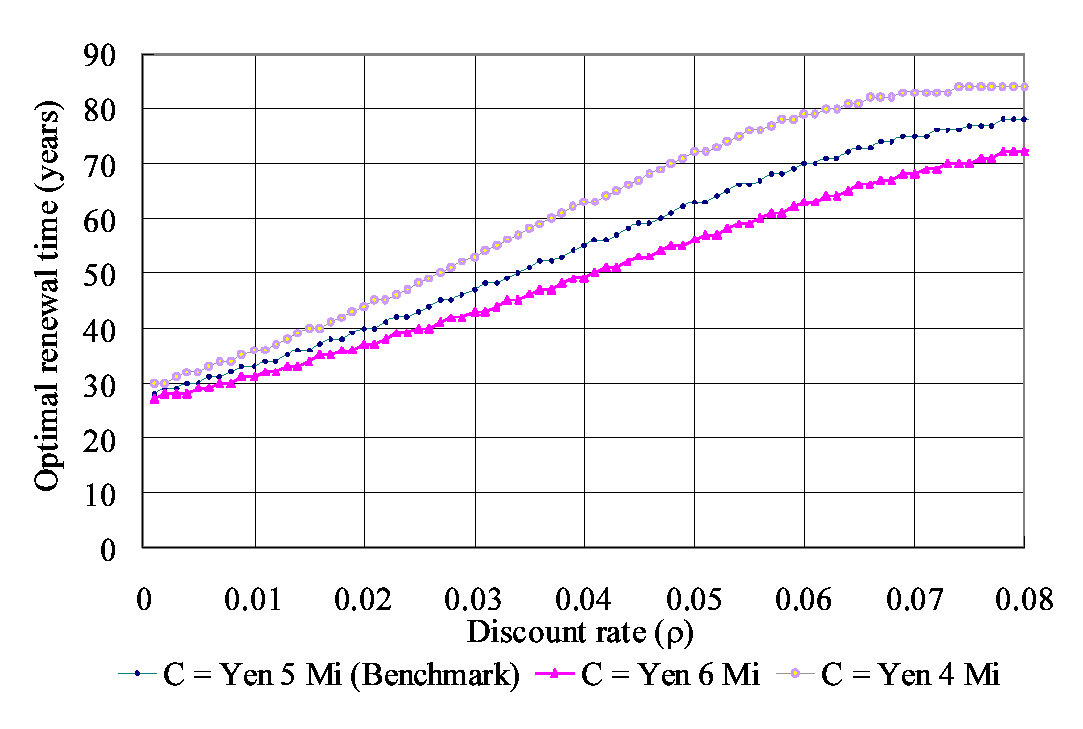
\includegraphics[scale=0.5]{fig58} 
\end{center}
\caption{Sensitivity Analysis-range of Discount Rate $\rho$.}
\label{fig58} 
\end{figure}
%
\begin{figure}[t]
\begin{center}
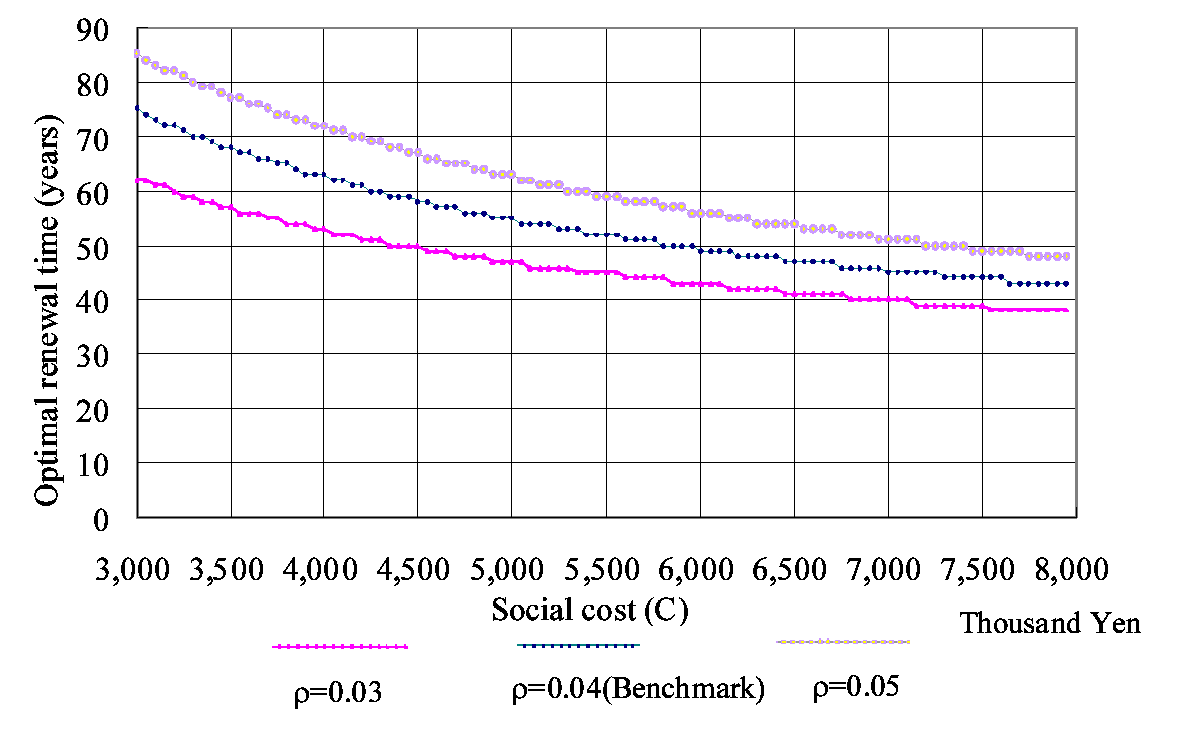
\includegraphics[scale=0.5]{fig59} 
\end{center}
\caption{Sensitivity Analysis-range of Social Cost $C$.}
\label{fig59} 
\end{figure}
%
\begin{figure}[t]
\begin{center}
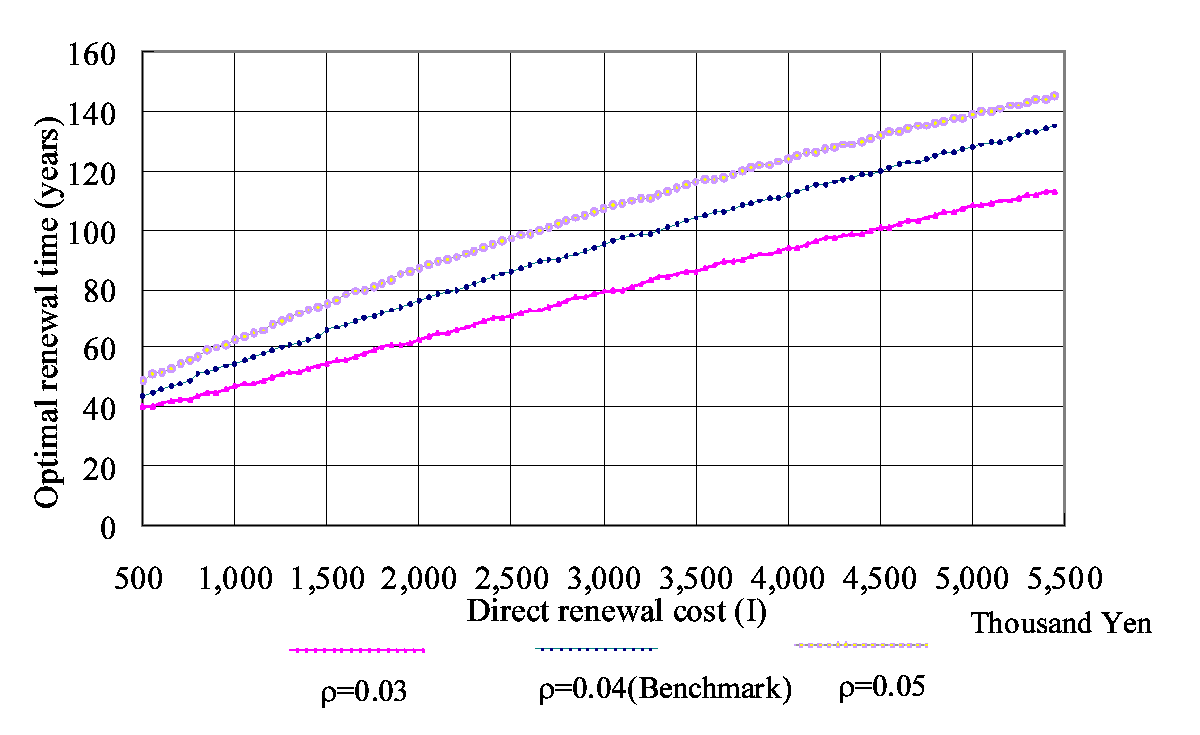
\includegraphics[scale=0.5]{fig510} 
\end{center}
\caption{Sensitivity Analysis-range of Direct Repair Cost $I$.}
\label{fig510} 
\end{figure}

Figure \ref{fig58} draws the change in optimal renewal years when changing the value of discount factor $\rho$. Benchmark optimal renewal duration curve is referred in the case of keeping $C$ = $5$ million Yen, $I$ = $1$ million Yen. Changing in value of either $C$ or $I$ consequently affects the optimal duration for renewal. For example, as can be seen from the figure, comparing to the benchmark case, increasing social cost $C$ = $1$ million relatively reduces the optimal duration about 3 to 10 years. Moreover, when $\rho$ becomes either very small (going close to $0$) nor large, convergence of optimal duration are obtained. Convergence of optimal duration is also realized when $\rho$ receives its value greater than $0.1$. High slope of optimal duration curve is acknowledged when $\rho$ $\le$ $0.05$.

The relationship between optimal renewal duration and change in social cost is sketched in Figure \ref{fig59}. It is realized that the increment in social cost results in the gradual shrink of optimal renewal duration. For example, if $500$ thousand Yen is added up to the benchmark case when keeping the same $I$ = $1$ million Yen and $\rho$ = $0.04$, the optimal duration is shortened about 6 to 10 years. 

Figure \ref{fig510} shows the correlation between optimal renewal duration and change in value of direct repair cost $I$. The linear rise of the curve proves a fact that higher direct repair cost leads to higher optimal renewal duration. For benchmark case ($C$ = $5$ million Yen, $I$ = $1$ million yen and $\rho$ = $0.04$), if happening the increase of $500$ thousand Yen in $I$, the optimal renewal duration goes up about 3 to 10 years. In the case when changing the discount factor $\rho$, it is found that the lower value of discount factor is, the smaller variation of optimal duration becomes.

In the case of using average cost analysis, the changes of optimal renewal years against social cost and direct renewal cost are plotted in Figure \ref{fig511}. In this Figure, we assume a constant value of direct cost $I=1$ million Yen when social cost change in the range from $1$ Million Yen to $20$ Million Yen. On the other hand, when direct cost $I$ changes, the social cost $C$ is assumed to equal to $5$ Million Yen. All relative costs are approximately calculated for pipelines with relative length of $140$ m. It is noted from this point that, the range of assumption value for either social cost and direct cost can be changed depending on various local conditions where analysis is deem applicable.
\begin{figure}[t]
\begin{center}
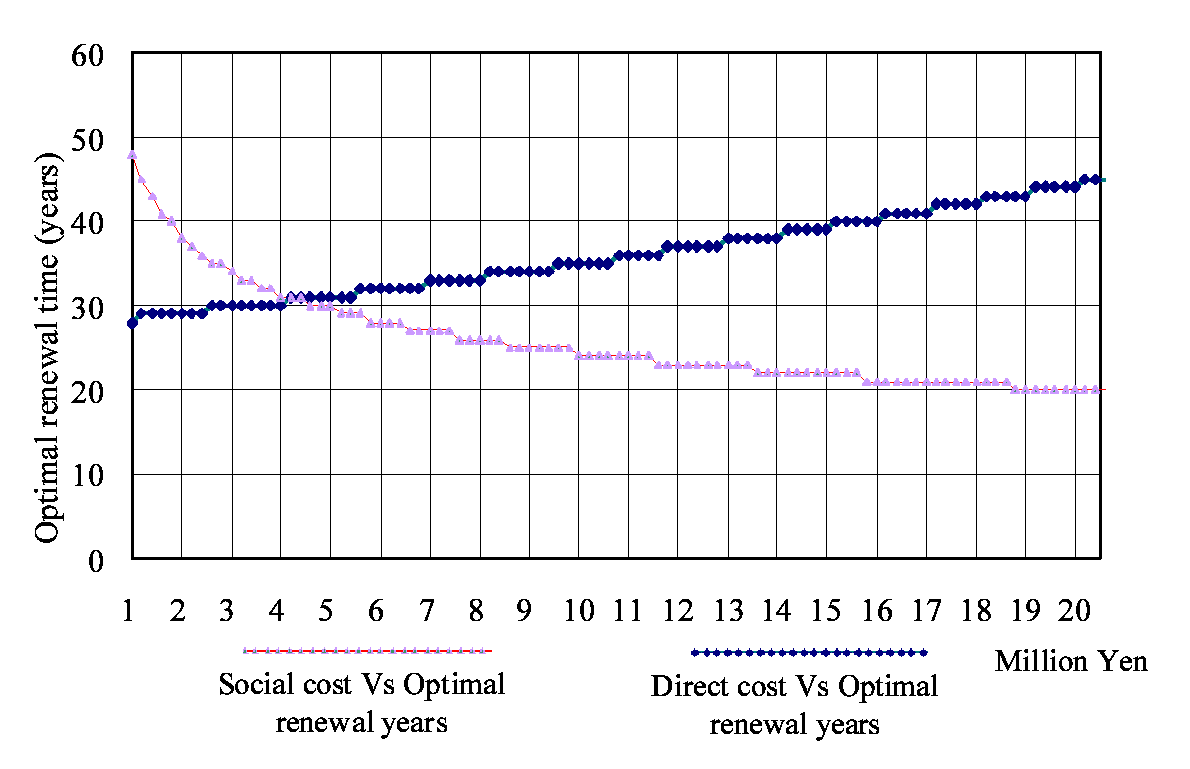
\includegraphics[scale=0.5]{fig511} 
\end{center}
\caption{Sensitivity Analysis - Average Cost.}
\label{fig511} 
\end{figure}
%%%%%%%%%%%%%%%%%%%%%%%%%%%%%%%%%%%%%%%%%%%%%%
\section{Summary and Recommendations}
\label{59}
%%%%%%%%%%%%%%%%%%%%%%%%%%%%%%%%%%%%%%%%%%%%%%
This chapter has presented a methodology to estimate the optimal renewal time of pipeline systems. The Weibull hazard function was employed to evaluate the survival probability of each types of pipeline with respect to the diameter. The mathematical formulation for calculating the total expected life cycle cost was introduced. The total expected life cycle cost took into account social cost and direct renewal cost in the event of leakage or breakdown of the pipeline. A system of water distribution network is comprised of many types of pipe materials, some of which might better be replaced to the optimal type of pipeline with pre-determined plan according to their forecasted survival probability. This is of crucial importance to uphold the safety level of the entire system, especially in the mega cities. 

An empirical application of the model to the water supply pipeline system in Osaka city was carried out. Results of the estimation identified the optimal renewal time for each type of pipeline. Sensitivity analysis reveals social cost $C$ and discount factor $I$ as important input factors of the model. These two values should be thoughtfully calculated for a more accurate outcome of optimal renewal time and concerning LCC. From the application view point, this model can be applied not only to water distribution networks but also to other types of underground infrastructure system.